\chapter{Implementacja i działanie systemu Team Challenge}

Lorem ipsum

\section{Środowisko implementacji}

Implementacja systemu odbywała się przy użyciu komputera wyposażonego w 8GB pamięci fizycznej oraz cztero-rdzeniowy procesor Intel Core i5-6300HQ (taktowanie 2.30GHz). Sprzęt o przytoczonych parametrach okazał się w pełni wystarczający dla przebiegu implementacji oraz lokalnego uruchamiania serwera aplikacji. Systemem operacyjnym używanym przy implementacji był Windows w wersji 10 Education. Wszystkie użyte programy i narzędzia dobrze współpracują z tym systemem.

\begin{table}[H]
\centering\small
\caption{Zestawienie narzędzi wykorzystywanych podczas implementacji systemu}
\label{tab:szablon}
\begin{tabularx}{\linewidth}{|p{.2\linewidth}|p{.1\linewidth}|p{.1\linewidth}|X|}\hline
Nazwa programu & Wersja & Producent & Cel\\ \hline\hline

IntelliJ IDEA & 2018.2 & Jetbrains & Implementacja aplikacji serwerowej (Java) \\ \hline

Webstorm & 2018.2 & Jetbrains & Implementacja aplikacji klienckiej (Angular) \\ \hline

Postman & 6.5.2 & Postman & Testowanie końcówek RESTowych aplikacji serwerowej \\ \hline

Google Chrome & 70 & Google & Testowanie aplikacji klienckiej \\ \hline

Git & 2.18.0 & - & Kontrola wersji \\ \hline

\end{tabularx}
\end{table}

\section{Implementacja aplikacji serwerowej}

\subsection{Struktura projektu}

Podstawowy szkielet projektu został utworzony przy użyciu Spring Initializr. Jako narzędzie służące do zarządzania zależnościami oraz budowy projektu wybrany został Apache Maven. 

\begin{comment}
W tabeli zostały przedstawione wykorzystane moduły Springa oraz inne biblioteki. 
\end{comment}

  Klasy tworzące aplikację serwerową zostały podzielone na pakiety pod względem tematycznym, co zaprezentowano na rysunku~\ref{fig:packages}. Podział taki pozwala na utrzymanie płaskiej struktury katalogów, a w związku z tym umożliwia szybkie odnajdywanie pożądanych plików.
  
  
\begin{figure}[ht]
\centering
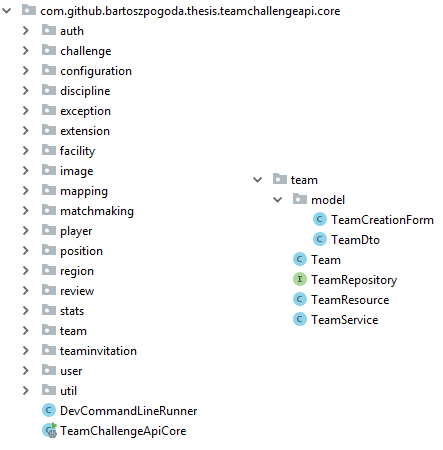
\includegraphics[width=0.5\linewidth]{06-implementacja/rys/package-team.PNG}
\caption{Fragment struktury pakietów}
\label{fig:packages}
\end{figure}

\subsection{Architektura wielowarstwowa}

Podczas projektowania architektury aplikacji ważne jest aby była ona przejrzysta oraz otwarta na rozszerzanie. Jedną z cech, którą powinny posiadać komponenty dobrze zaprojektowanego oprogramowania zorientowanego obiektowo jest ograniczenie odpowiedzialności. Jedną z metod rozdzielania odpowiedzialności jest wyszczególnienie w projekcie warstw komponentów. Aplikacja serwerowa będąca przedmiotem niniejszej pracy została podzielona na warstwy zgodnie ze standardami zdefiniowanymi dla szkieletu Spring. Wyszczególnione warstwy wraz z kierunkami komunikacji zostały przedstawione na rysunku~\ref{fig:app-layers}.


\begin{comment}

Nawiazanie do: 
Understanding Spring Web Application Architecture: The Classic Way
Petri Kainulainen October 19, 2014
https://www.petrikainulainen.net/software-development/design/understanding-spring-web-application-architecture-the-classic-way/

\end{comment}

\begin{figure}[H]
\centering
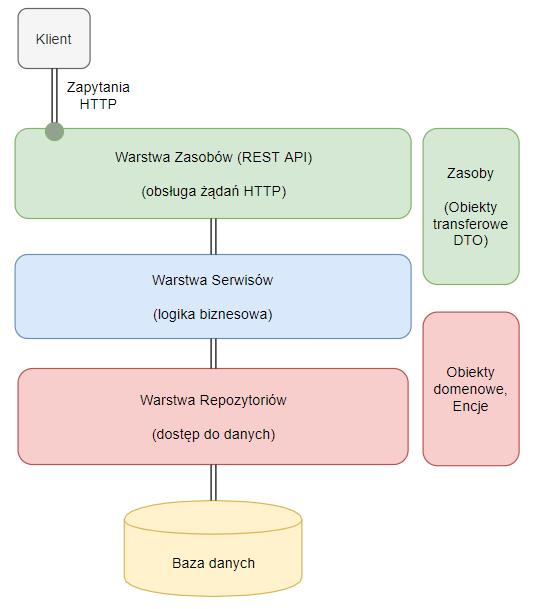
\includegraphics[width=0.5\linewidth]{06-implementacja/rys/layers.PNG}
\caption{Warstwy aplikacji serwerowej}
\label{fig:app-layers}
\end{figure}


\subsection{Warstwa repozytoriów}

Repozytoria w frameworku Spring stanowią mechanizm dostępu do danych. Warstwa ta jest abstrakcją ukrywającą przed programistą szczegóły komunikacji z bazą danych takie jak: nawiązywanie oraz utrzymywanie połączenia, konstrukcja i wykonywanie zapytań, mapowanie wyników. Deklaracja fizycznych powiązań między aplikacją a bazą danych odbywa się za pomocą adnotacji. Na listingu~\ref{list:entity} przedstawiono powiązanie encji Team z fizyczną tabelą o nazwie Teams oraz mapowania przykładowych kolumn.

\begin{lstlisting}[label=list:entity, caption=Fragment przykładowej encji, basicstyle=\footnotesize\ttfamily]
@Entity
@Table(name = "Teams")
@Data
@Builder
public class Team {

    @Id
    @GeneratedValue(strategy = GenerationType.IDENTITY)
    @Column(name = "TeamID")
    private String id;

    @OneToOne(fetch = FetchType.EAGER)
    @JoinColumn(name = "ManagerID")
    private Player manager;

    @OneToMany(mappedBy = "team", cascade = CascadeType.ALL)
    private List<Player> players;
    
    // other fields with their mappings...
}
\end{lstlisting}

Dostęp do danych zapewniają repozytoria, czyli interfejsy oznaczone adnotacją @Repository. Wygodne jest rozszerzanie dostarczonego przez moduł Spring Data interfejsu CrudRepository, który definiuje podstawowe metody dostępu takie jak dodawanie, czytanie, modyfikacja oraz usuwanie encji. Pozostałe metody potrzebne do realizacji logiki biznesowej można definiować poprzez tworzenie metod o nazwach specyfikujących ich działanie. Fizyczne zapytania do bazy danych wyznaczane są na podstawie nazwy metody. Przykładową definicję repozytorium przedstawiono na listingu~\ref{list:repository}.

\begin{lstlisting}[label=list:repository, caption=Definicja przykładowego repozytorium, basicstyle=\footnotesize\ttfamily]
@Repository
public interface TeamRepository 
extends CrudRepository<Team, String>, JpaSpecificationExecutor<Team> {

    Optional<Team> findById(String id);

    List<Team> findByRegionIdAndDisciplineIdAndActiveIsTrue(String regionId,
     String disciplineId);
}
\end{lstlisting}

Dostarczenie interfejsu repozytorium rozszerzającego JpaSpecificationExecutor pozwala na wykonywanie bardziej zaawansowanych zapytań. Mechanizm ten został zastosowany przy tworzeniu zapytań, gdzie lista predykatów była ustalana w zależności od parametrów zapytania HTTP w sposób dynamiczny. Do budowy kwerend użyto klas Specification oraz Predicate pochodzących z modułu Sring Data JPA.


\subsection{Warstwa serwisów}

Podstawowym zadaniem serwisów jest przetwarzanie danych zgodnie z regułami biznesowymi. W zaimplementowanym systemie na poziomie serwisów również sprawdzane są prawa dostępu do zasobów. W Springu serwisy oznaczane są adnotacje @Service. Framework sam zajmuje się tworzeniem instancji serwisów, które mogą być użyte w pozostałych komponentach systemu. Przykładowy serwis został przedstawiony na listingu~\ref{list:service}.

\begin{comment}
Możę o wstrzykiwaniu zależności tutaj.
\end{comment}

\begin{minipage}{\linewidth}
\begin{lstlisting}[label=list:service, caption=Fragment przykładowego serwisu, basicstyle=\footnotesize\ttfamily]

@Service
public class TeamService {

    private TeamRepository teamRepository;
    private PositionService positionService;
    // other fields...
    
    @Transactional
    public Position setHome(String id, PositionDto positionDto) 
    	throws TeamNotFoundException, AccessForbiddenException {
    
        Team team = teamRepository.findById(id)
        .orElseThrow(TeamNotFoundException::new);
        
        if(!isManagedByCurrentUser(team)) {
            throw new AccessForbiddenException();
        }

        Position position = this.positionService.save(positionDto);
        team.setHome(position);

        return position;
    }
    
    // other methods...
}
\end{lstlisting}
\end{minipage}


\subsection{Warstwa zasobów}

Warstwa zasobów jest szczególna, z tego względu, że stanowi interfejs sytemu dla świata zewnętrznego. W ramach tej warstwy działa dostarczony przez szkielet Spring Dispatcher Servlet. Jest to komponent obsługujący żądania HTTP przychodzące do aplikacji. W ramach obsługi żądania są one przekazywane do konkretnych "kontrolerów", wybranych na podstawie URL żądania. Listing~\ref{list:resource}. przedstawia rejestracje kontrolera za pomocą adnotacji @RestController oraz @RequestMapping. Dispatcher Servlet w przypadku tak skonfigurowanej klasy będzie kierował zapytania o adresie /teams do kontrolera TeamResource. Zapytanie /teams/4  zostanie przekazane konkretnie do metody getTeam z argumentem wywołania równym 4.

Na poziomie warstwy zasobów odbywa się również walidacja przychodzących danych.

\begin{minipage}{\linewidth}
\begin{lstlisting}[label=list:resource, caption=Przykładowa rejestracja kontrolera, basicstyle=\footnotesize\ttfamily]

@RestController
@RequestMapping("/teams")
public class TeamResource {

    private TeamService teamService;

    private DtoMappingService mappingService;

    @GetMapping("/{id}")
    public ResponseEntity<TeamDto> getTeam(@PathVariable String id)
     throws ApiException {
        return teamService.findById(id)
                .map(mappingService::mapToDto)
                .map(ResponseEntity::ok)
                .orElseThrow(TeamNotFoundException::new);
    }
    
    // other methods ...
}

\end{lstlisting}
\end{minipage}

Pełna specyfikacja REST API została przedstawiona w załączniku X.

\subsection{Algorytm poszukiwania rywali}

Algorytm poszukiwania rywali został zaimplementowany w oparciu o zagadnienie optymalizacji wielokryterialnej, które zostało przybliżone w trzecim rozdziale niniejszej pracy. Podczas prac nad algorytmem uwzględniono domenę problemu oraz charakter danych, na jakich będzie on operował. W związku z tym tradycyjny schemat oceny decyzji został rozszerzony, co zostało opisane w dalszej części tego rozdziału. Rysunek~\ref{fig:diagram-alg-ext} przedstawia uproszczony schemat działania algorytmu zrealizowanego w systemie.

\begin{figure}[H]
\centering
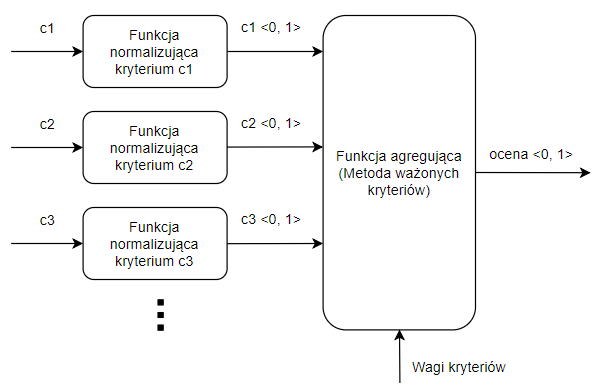
\includegraphics[width=0.8\linewidth]{03-koncept/rys/algorytm.PNG}
\caption{Schemat działania algorytmu oceny decyzji}
\label{fig:diagram-alg-ext}
\end{figure}

\subsubsection{Kryteria}

W systemie zostały wyszczególnione dwa główne rodzaje kryteriów - numeryczne oraz logiczne. Kryteria numeryczne obejmują kryteria, które da się zmierzyć i wyrazić w postaci liczbowej. Uwzględniono tutaj takie kryteria jak: różnica wieku, różnica umiejętności oraz odległość między drużynami. Kryteria logiczne wyrażają dodatkowe wskaźniki, które mają wpływ na dobre dopasowanie drużyn, jednak nie są policzalne.  Kryteriom tym przypisane są wartości logiczne, które oznaczają czy dane kryterium zostało spełnione. Przykładowo wartość logiczna kryterium dotyczącego poziomu fair play będzie ustawiona jeżeli średnia ocen fair play potencjalnych rywali jest większa lub równa 4 (maksymalnie 5).

Dodatkowo wyszczególniono generyczną klasę, która opakowuje dowolne kryterium dodając informację o znormalizowanej wartości liczbowej. 

Zastosowaną hierarchię klas przedstawiono na rysunku \ref{fig:criterion-classes}. Rozbudowa funkcjonalności o nowe kryteria sprowadza się do utworzenia dodatkowej implementacji w odpowiednim miejscu hierarchii.  

\begin{figure}[H]
\centering
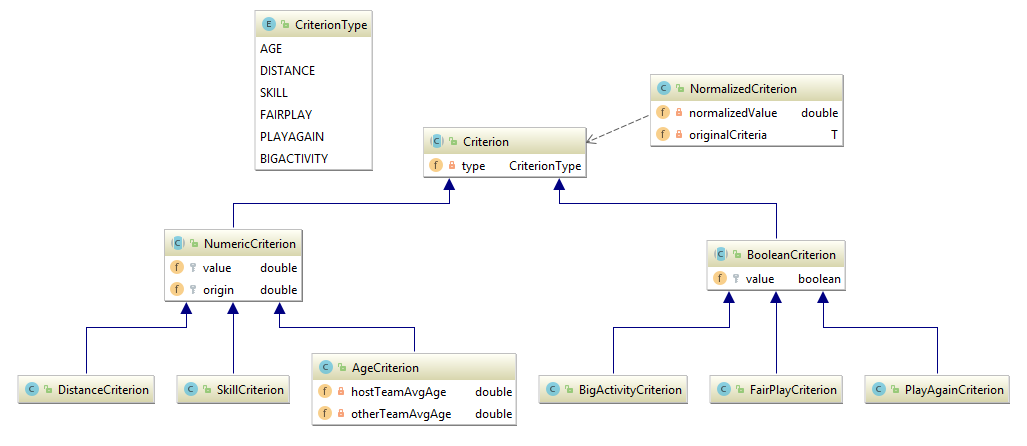
\includegraphics[width=\linewidth]{06-implementacja/rys/criterion-package-classes.PNG}
\caption{Hierarchia klas: kryteria}
\label{fig:criterion-classes}
\end{figure}

Kryteria dla poszczególnych decyzji generowane są na podstawie zgromadzonych danych o drużynach, zawodnikach oraz wynikach spotkań. Przykładową metodę przedstawiono na listingu \ref{list:age-crit-gen}. 


\begin{minipage}{\linewidth}
\begin{lstlisting}[label=list:age-crit-gen, caption=Generacja kryterium różnicy wieku między dwoma drużynami, basicstyle=\footnotesize\ttfamily]
public AgeCriterion ageCriteria(Team hostTeam, Team otherTeam) {
  double averageAgeHostTeam = hostTeam.getPlayers().stream()
                .mapToDouble(playerService::getAge).average().orElse(0);
  double averageAgeOtherTeam = otherTeam.getPlayers().stream()
                .mapToDouble(playerService::getAge).average().orElse(0);

  return new AgeCriterion(
    averageAgeOtherTeam - averageAgeHostTeam, 
    averageAgeHostTeam, 
    averageAgeOtherTeam
  );
}
\end{lstlisting}
\end{minipage}

\subsubsection{Normalizacja kryteriów}

 Normalizacja poszczególnych kryteriów przebiega przy użyciu różnych funkcji, dopasowanych do charakteru danych. Przykładem uzasadniającym konieczność zastosowania takiej modyfikacji może być porównanie dwóch kryteriów: odległości drużyn oraz średniego wieku zawodników. O ile kryterium odległości może być normalizowane w pełni liniowo, o tyle dla różnicy wieku taka metoda normalizacji jest błędna. Różnica wieku między dwoma zawodnikami, którzy mają 15 oraz 20 lat jest znacznie bardziej istotna aniżeli różnica między zawodnikami w wieku 30 oraz 35 lat - nie można tutaj zastosować operatora w pełni liniowego. Dodatkowo w domenie problemu wyróżniono kryteria nieliczbowe - cechy drużyny, które mogą mieć duży wpływ na jakość dopasowania, np. zadeklarowana chęć ponownej gry z daną drużyną.  
 
 \begin{comment}
O metodach normalizacji - LinearDecay itp. 
 \end{comment}
 
\begin{figure}[H]
\centering
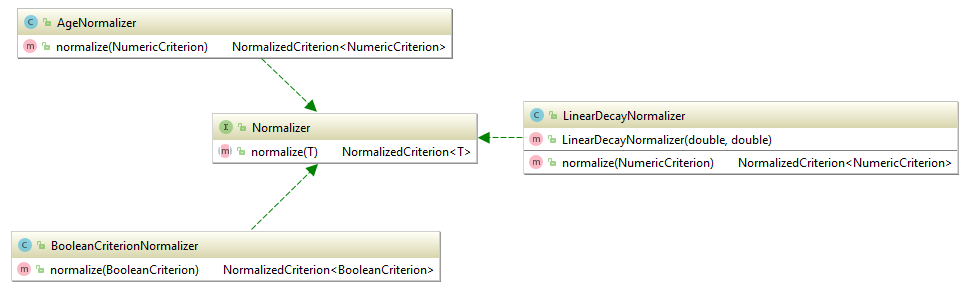
\includegraphics[width=\linewidth]{06-implementacja/rys/normalizer-hierarchy.PNG}
\caption{Hierarchia klas: normalizacja}
\label{fig:criterion-classes}
\end{figure}

\subsubsection{Metoda ważonych kryteriów}

Metoda ważonych kryteriów polega na opisaniu funkcji oceny decyzji jako sumy ważonej ocen poszczególnych kryteriów \cite{analizawielok}. Konieczne jest przyporządkowanie wagi dla każdego z kryteriów. Ocena poszczególnych decyzji obliczana jest według wzoru: 

\begin{equation}\label{eq:mwk}
F(x)=\sum_{i=1}^{k}w_{i}f_{i}(x)
\end{equation}

gdzie k - ilość kryteriów, x - wektor rozwiązań, $w_{i}$ - wagi takie że:

\begin{equation*}
w \in [0, 1] \mbox{ oraz } \sum_{i=1}^{k}w_{i} = 1
\end{equation*}

Metoda ta została wybrana ze względu na możliwość dynamicznego doboru wag poszczególnych kryteriów. Niektóre z tych wag będą dobierane przez kapitana zgodnie z preferencjami jego drużyny. 


\begin{minipage}{\linewidth}
\begin{lstlisting}[label=list:resource, caption=Przykładowa rejestracja kontrolera, basicstyle=\footnotesize\ttfamily]

@Service
public class WeightedCriteriaAggregator {

    public double aggregate(List<WeightedCriteria> weightedCriteria) {
      return aggregate(weightedCriteria.stream());
    }

    public double aggregate(Stream<WeightedCriteria> stream) {
      return stream
      .mapToDouble(
       crit -> crit.getWeight() * crit.getCriteria().getNormalizedValue()
       )
      .sum();
    }

}

\end{lstlisting}
\end{minipage}

\section{Implementacja aplikacji klienckiej}

\subsection{Modularność}

Podobnie jak aplikacja serwerowa, aplikacja kliencka została zrealizowana w architekturze ograniczającej odpowiedzialność poszczególnych komponentów. W technologii Angular modularność uzyskuję się poprzez podział na komponenty oraz moduły, które je agregują w zbiory [X]. 

Istotnym wzorcem jaki został zastosowany w projekcie jest dodatkowy podział komponentów na komponenty prezentacyjne oraz kontenery. Komponenty prezentacyjne zajmują się jedynie wyświetlaniem danych przekazanych im na wejściach oraz pobieraniem danych od użytkownika i przekazywaniem ich na wyjścia. Kontenery posiadają większy zakres odpowiedzialności - znają stan aplikacji oraz mogą na niego wpływać. Kontenery używają komponentów prezentacyjnych do interakcji z użytkownikiem [X]. Zastosowanie takiego podziału usprawniło rozwój aplikacji oraz pozwoliło na używanie raz zaimplementowanych komponentów prezentacyjnych w różnych miejscach aplikacji.

\begin{comment}
Angular Docs:  Architecture overview
https://angular.io/guide/architecture

https://blog.angular-university.io/angular-2-smart-components-vs-presentation-components-whats-the-difference-when-to-use-each-and-why/
Angular Architecture - Smart Components vs Presentational Components
18 JUNE 2018
Angular Unversity
\end{comment}



\begin{figure}[H]
\centering
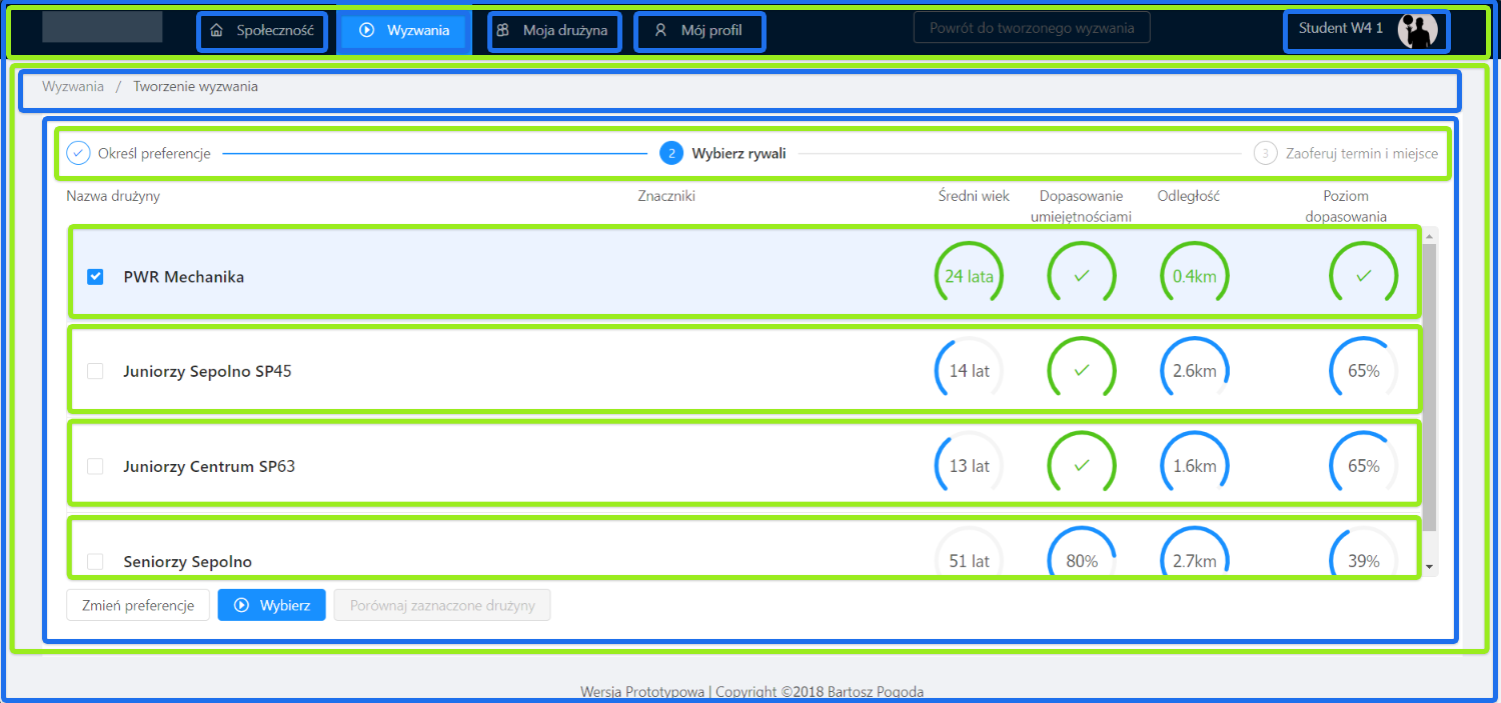
\includegraphics[width=\linewidth]{06-implementacja/rys/modularyzacja.PNG}
\caption{Widok wyników poszukiwania rywali: Podział na komponenty}
\label{fig:criterion-classes}
\end{figure}


\subsection{Stan aplikacji}

Jednym z wyzwań podczas implementacji aplikacji działających w przeglądarce jest zarządzanie ich stanem. Tradycyjnym podejściem dla aplikacji w technologii Angular jest przetrzymywanie danych w komponentach oraz serwisach. Sposób ten działa bez zarzutów dla bardzo małych aplikacji, jednak w miarę rozwoju pojawiają się problemy takie jak: przekazywanie danych pomiędzy komponentami, które nie zależą bezpośrednio od siebie oraz problemy z synchronizacją danych. Drugi problem dotyczy sytuacji, w której dwa komponenty korzystają z tych samych obiektów, a w pewnym momencie okazuje się, że obiekty te są różne. Ciężko jest stwierdzić, który komponent zawiera referencje do obiektu prawdziwego - aktualnego. Rozwiązaniem opisanych problemów jest wdrożenie do aplikacji koncepcji \textit{Store}. Podejście to polega na przetrzymywaniu stanu aplikacji w jednym obiekcie. Eliminuje to problem konfliktów, w aplikacji występuje tylko jedno źródło prawdy (ang. \textit{Source of truth}). Korzystanie przez różne komponenty z tych samych danych również staje się proste ze względu na przetrzymywanie ich w centralnym miejscu dostępnym z każdego miejsca aplikacji.

Warto również dodać, że stan aplikacji jest obiektem niemodyfikowalnym. Jedynym sposobem na zmianę stanu jest zmiana referencji na nowy obiekt. W opisywanej architekturze zajmują się tym specjalne funkcje redukujące. Funkcje te na podstawie zgłaszanych akcji dokonują aktualizacji stanu. Akcje są zgłaszane w momencie zdarzeń wygenerowanych przez użytkownika, zewnętrzne systemy bądź wewnętrznie w aplikacji. Jedną z głównych zalet takiego sposobu zmian stanu jest zwiększenie wydajności aplikacji w technologii \textit{Angular}. Komponenty mogą korzystać z bardzo wydajnego trybu odświeżania, który aktualizuje widok jedynie w momencie zmiany referencji podanych na jego wejścia - co ma miejsce przy aktualizacjach w zastosowanej architekturze. Kolejną równie ważną zaletą jest znaczne ułatwienie wykrywania błędów oraz ich przyczyn. Istnieją narzędzia deweloperskie pozwalające na śledzenie stanu  oraz jego zmian podczas działania aplikacji. Przykładowy podgląd części stanu w formie drzewa przedstawiono na rysunku \ref{fig:state}. Narzędzia umożliwiają również podgląd obiektu stanu w formacie \textit{JSON}. Przykładową sekwencję akcji generowanych oraz obsługiwanych przy logowaniu do aplikacji ukazano na rysunku \ref{fig:actions}.

\begin{figure}[H]
\centering
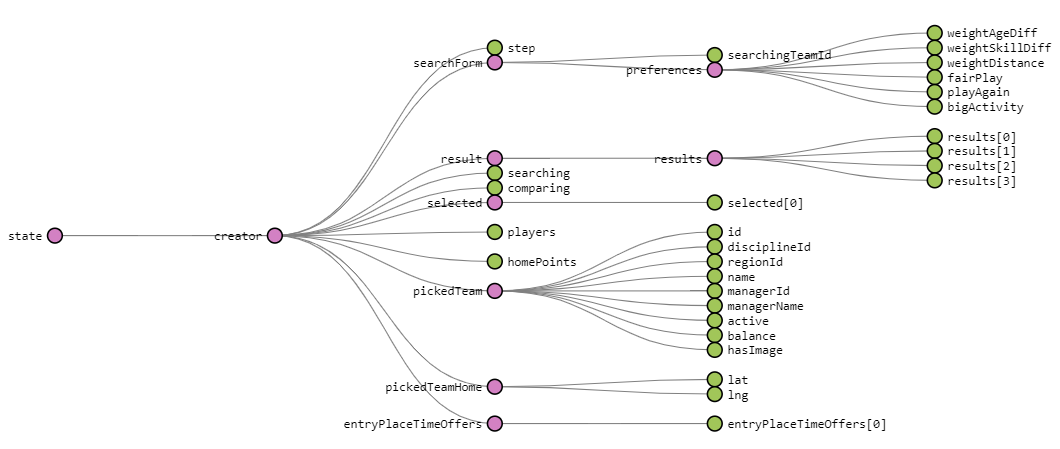
\includegraphics[width=\linewidth]{06-implementacja/rys/state-after.PNG}
\caption{Przykładowy fragment drzewa stanu aplikacji}
\label{fig:state}
\end{figure}


\begin{figure}[H]
\centering
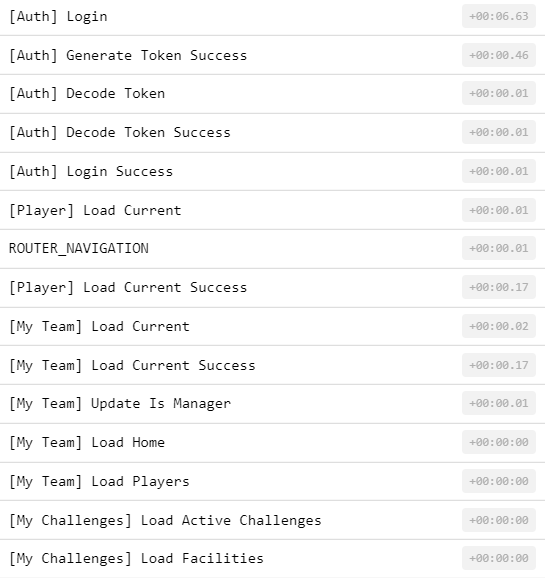
\includegraphics[width=0.5\linewidth]{06-implementacja/rys/actions.PNG}
\caption{Przykładowa sekwencja akcji przy logowaniu do aplikacji}
\label{fig:actions}
\end{figure}


\subsection{Formularze}

Wiele funkcjonalności Team Challenge opiera się na pobraniu danych od użytkowników. W technologii \textit{Angular} wyróżnia się dwa główne sposoby budowy formularzy - sterowane znacznikami \textit{HTML} oraz reaktywne (ang. \textit{reactive}). Podczas implementacji systemu użyto formularzy reaktywnych. Są one zalecane przez twórców szkieletu \textit{Angular} ze względu na większą skalowalność oraz możliwości wielokrotnego użytku. 

Komponenty wizualne takie jak przyciski, suwaki oraz pola tekstowe zostały dostarczone przez bibliotekę \textit{NgZorro}. 


\begin{comment}


https://angular.io/guide/forms-overview

kontrolki od zorro, step forms, store
formularze, Walidacja formularzy, pare screenow, odowlanie do instrukcji uzytkownika w zalaczniku

\end{comment} 



\begin{figure}[H]
\centering
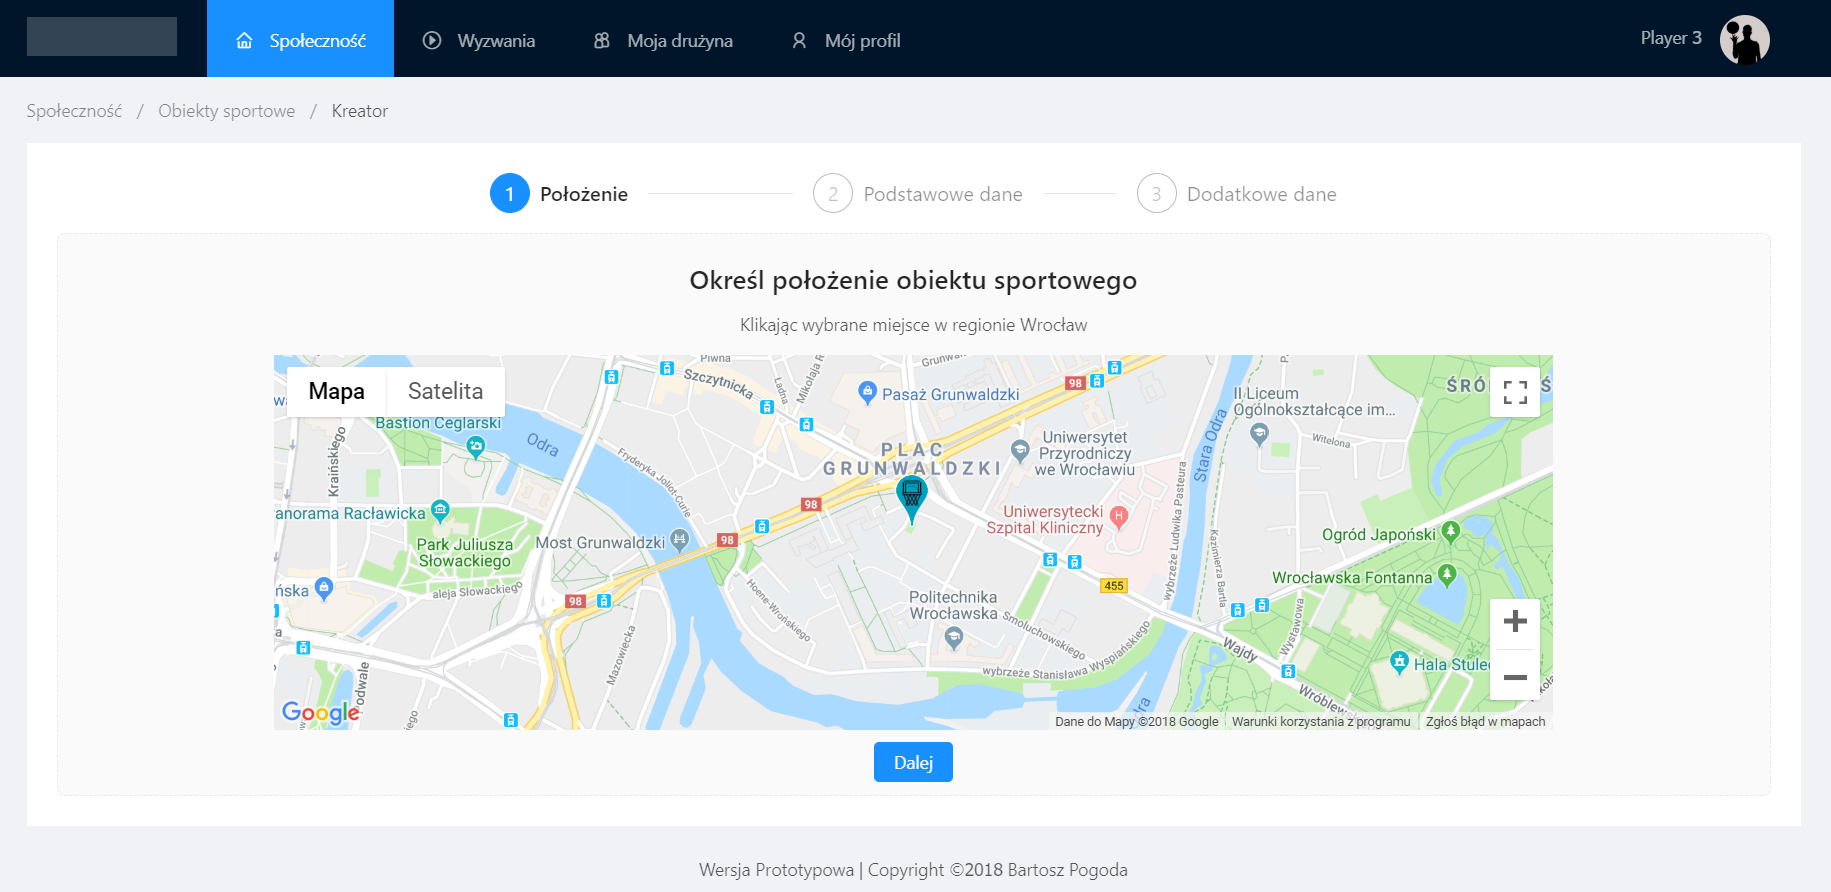
\includegraphics[width=\linewidth]{06-implementacja/rys/form1.PNG}
\caption{Formularz wprowadzania obiektu sportowego - Krok pierwszy}
\label{fig:sample-form}
\end{figure}



\begin{figure}[H]
\centering
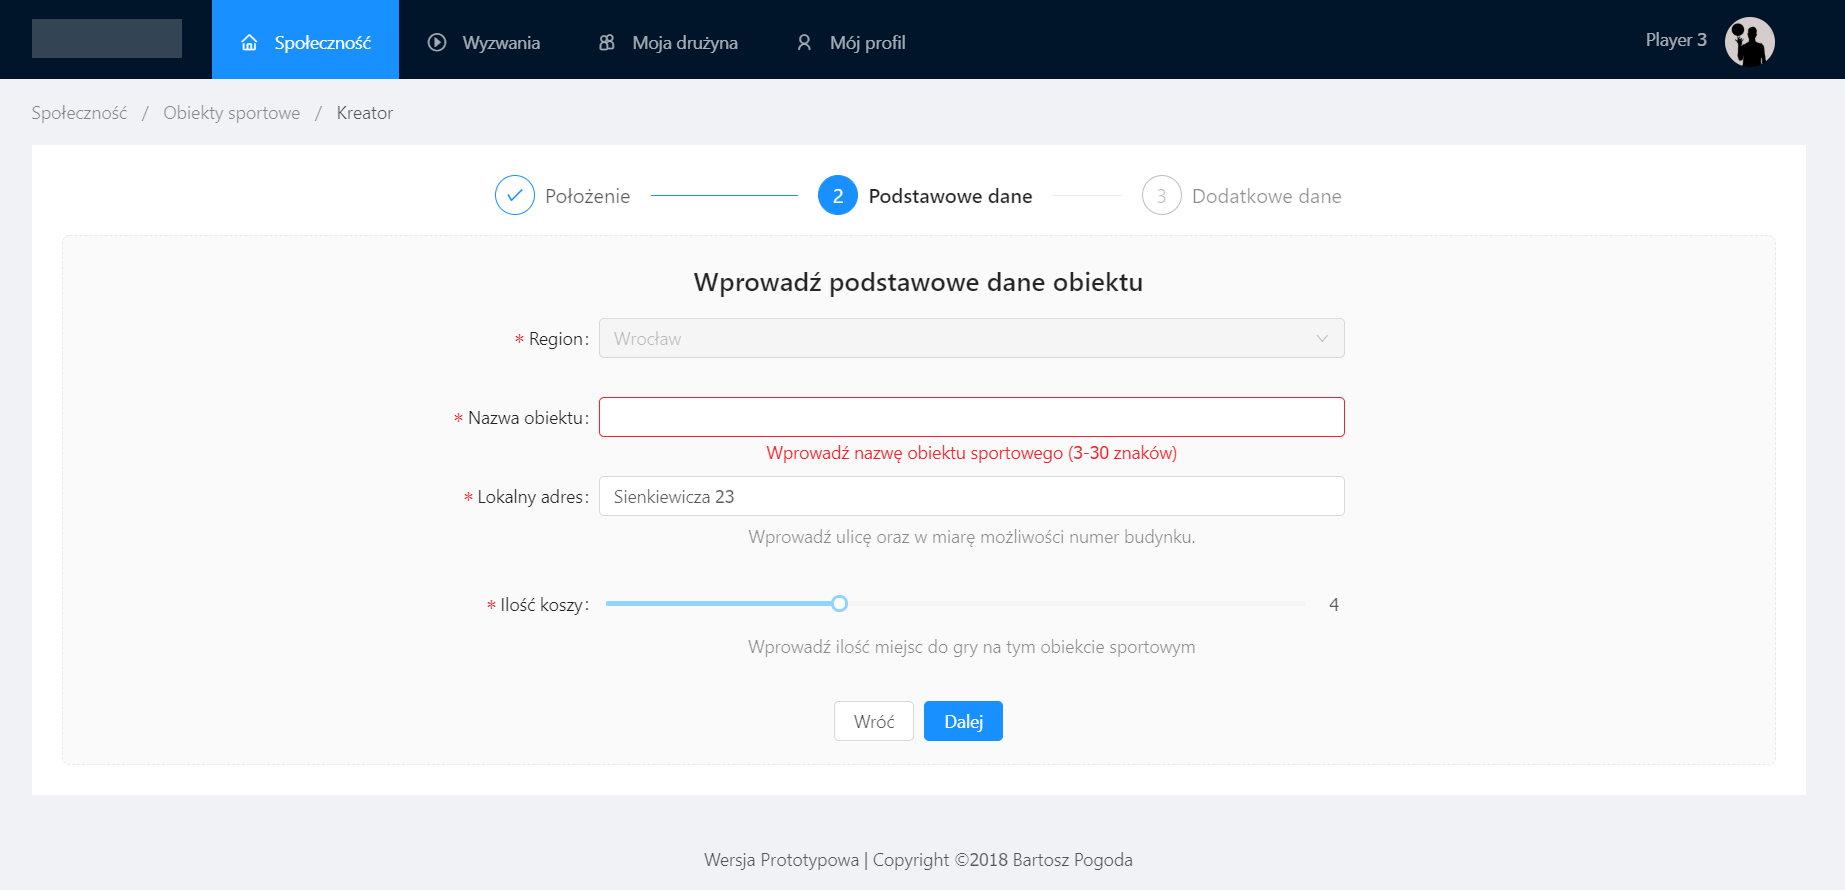
\includegraphics[width=\linewidth]{06-implementacja/rys/form2.PNG}
\caption{Formularz wprowadzania obiektu sportowego - Krok drugi}
\label{fig:sample-form}
\end{figure}




\begin{figure}[H]
\centering
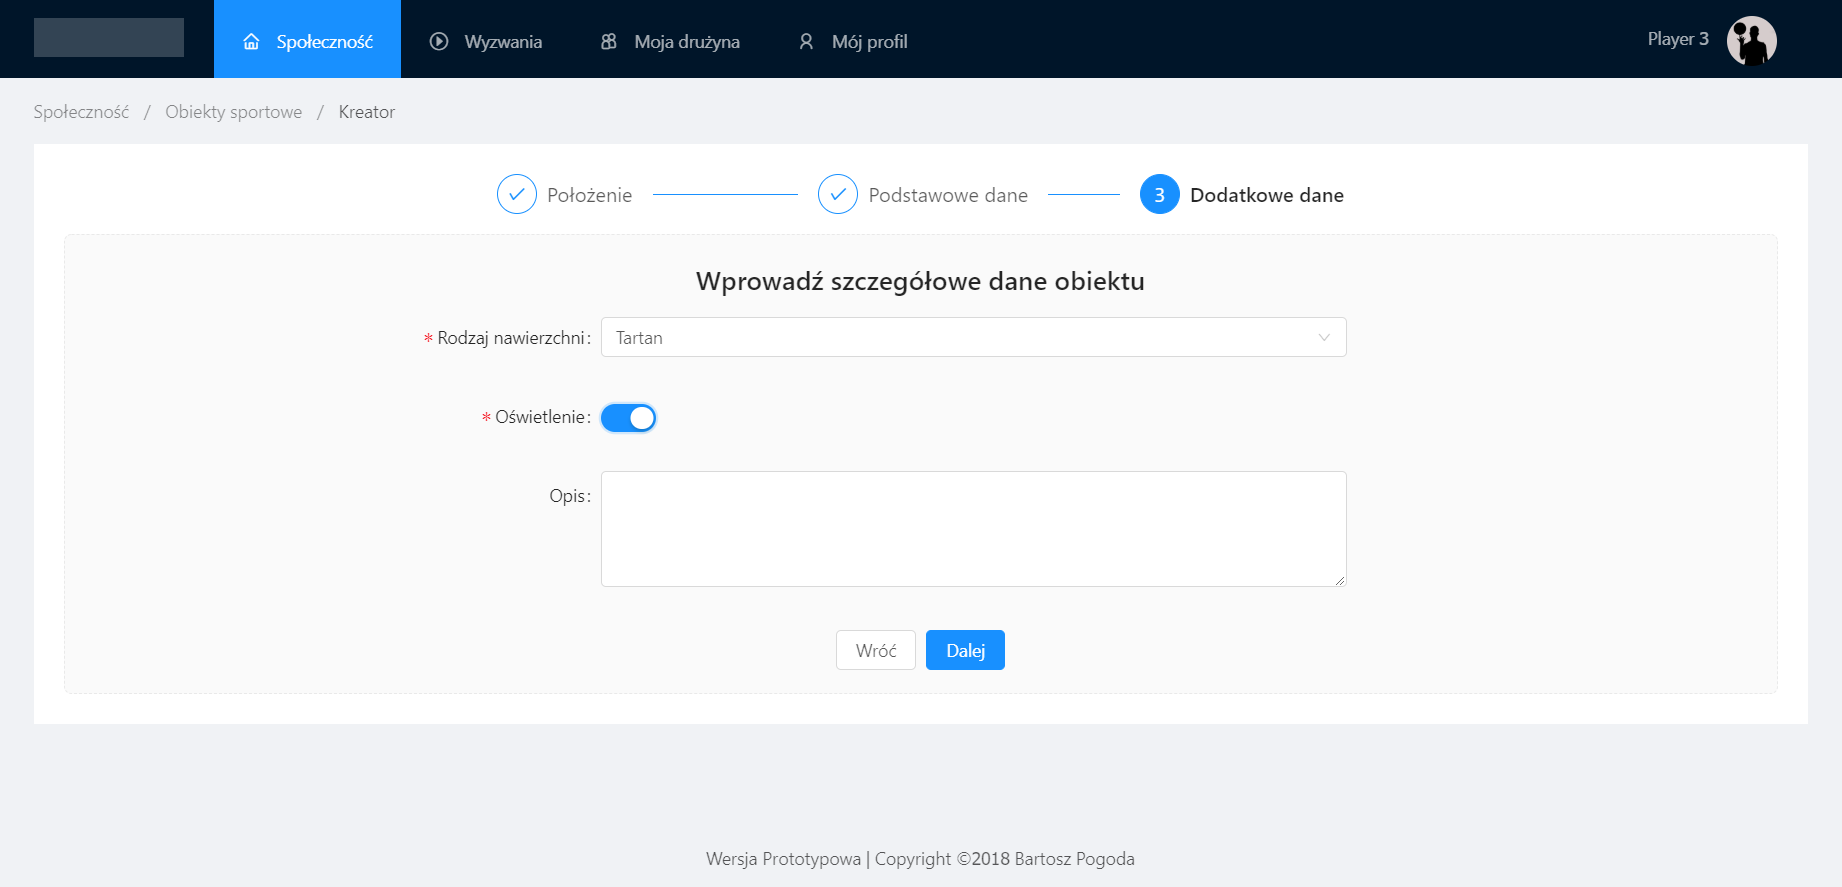
\includegraphics[width=\linewidth]{06-implementacja/rys/form3.PNG}
\caption{Formularz wprowadzania obiektu sportowego - Krok trzeci}
\label{fig:sample-form}
\end{figure}


\section{Bezpieczeństwo}

Szczególną uwagę poświęcono implementacji zabezpieczeń systemu oraz zgromadzonych danych użytkowników. Funkcjonalności związane z bezpieczeństwem zostały zrealizowane bazując na module Spring Security, który dostarcza wiele przydatnych mechanizmów oraz możliwości ich konfiguracji.

Hasła użytkowników przechowywane są w formie zaszyfrowanej za pomocą funkcji skrótu BCrypt. Spring Security dostarcza klasę implementującą ten algorytm - BCryptPasswordEncoder. Główną zaletą takiego sposobu szyfrowania jest generowanie losowego ciągu znaków, tak zwanej soli, który dodatkowo wzmacnia bezpieczeństwo hasła. Zastosowanie soli przy hashowaniu znacznie utrudnia złamanie hasła przez ataki przy użyciu tęczowych tabel. W przypadku algorytmu bcrypt wygenerowana sól jest przechowywana razem z zaszyfrowanym hasłem w bazie danych. W przypadku prób logowania jest ona wyciągana z bazy oraz używana do przetworzenia podanego hasła w celu porównania zgodności.


Autoryzacja zapytań (JWT)


\begin{figure}[H]
\centering
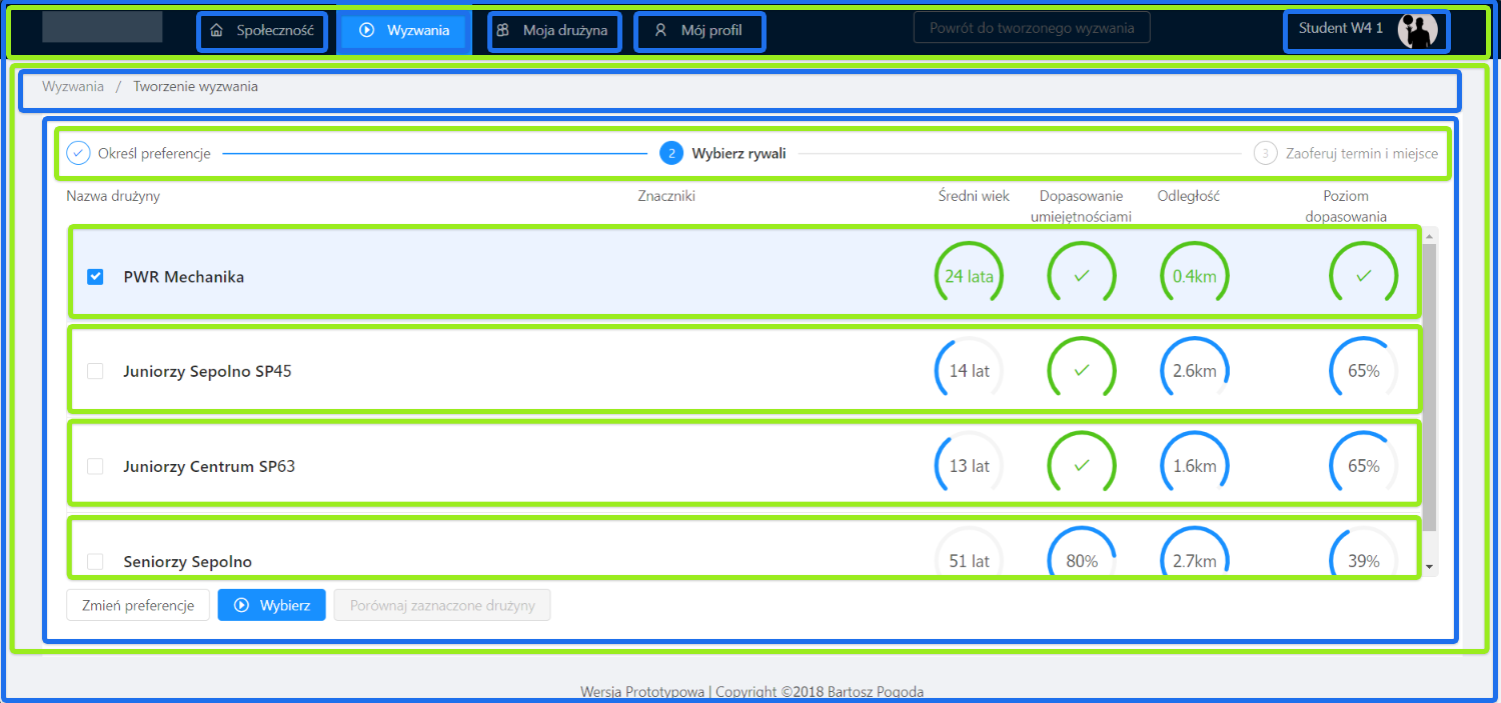
\includegraphics[width=0.7\linewidth]{06-implementacja/rys/modularyzacja.PNG}
\caption{Hierarchia klas: normalizacja}
\label{fig:criterion-classes}
\end{figure}